\documentclass[../thesis.tex]{subfiles}

\begin{document}
\chapter{System Overview}
\label{chap:syso}

\section{Concept}


\subsection{Monitoring}
The solar panel generates electricity and feeds it into the converter after being measured by the current and voltage sensor. The converter converts the electricity from a higher voltage to the desired voltage, which can be measured again by the sensor and used to charge the battery. The sensing data consist of input current and voltage and output current and voltage, which are fed into the microcontroller. The microcontroller has a 4G cellular modem which enables communication with the surrounding 4G cellular base station, and the internet access is provided by the gateway at the base station. That means the sensing data can be sent from the microcontroller to the server through the 4G cellular network. Once the sensing data reaches the server, the data is processed, store into the database, and send to the client such as a web application. The concept for monitoring is shown in figure \ref{fig:concept1}.

\begin{figure}[!ht]
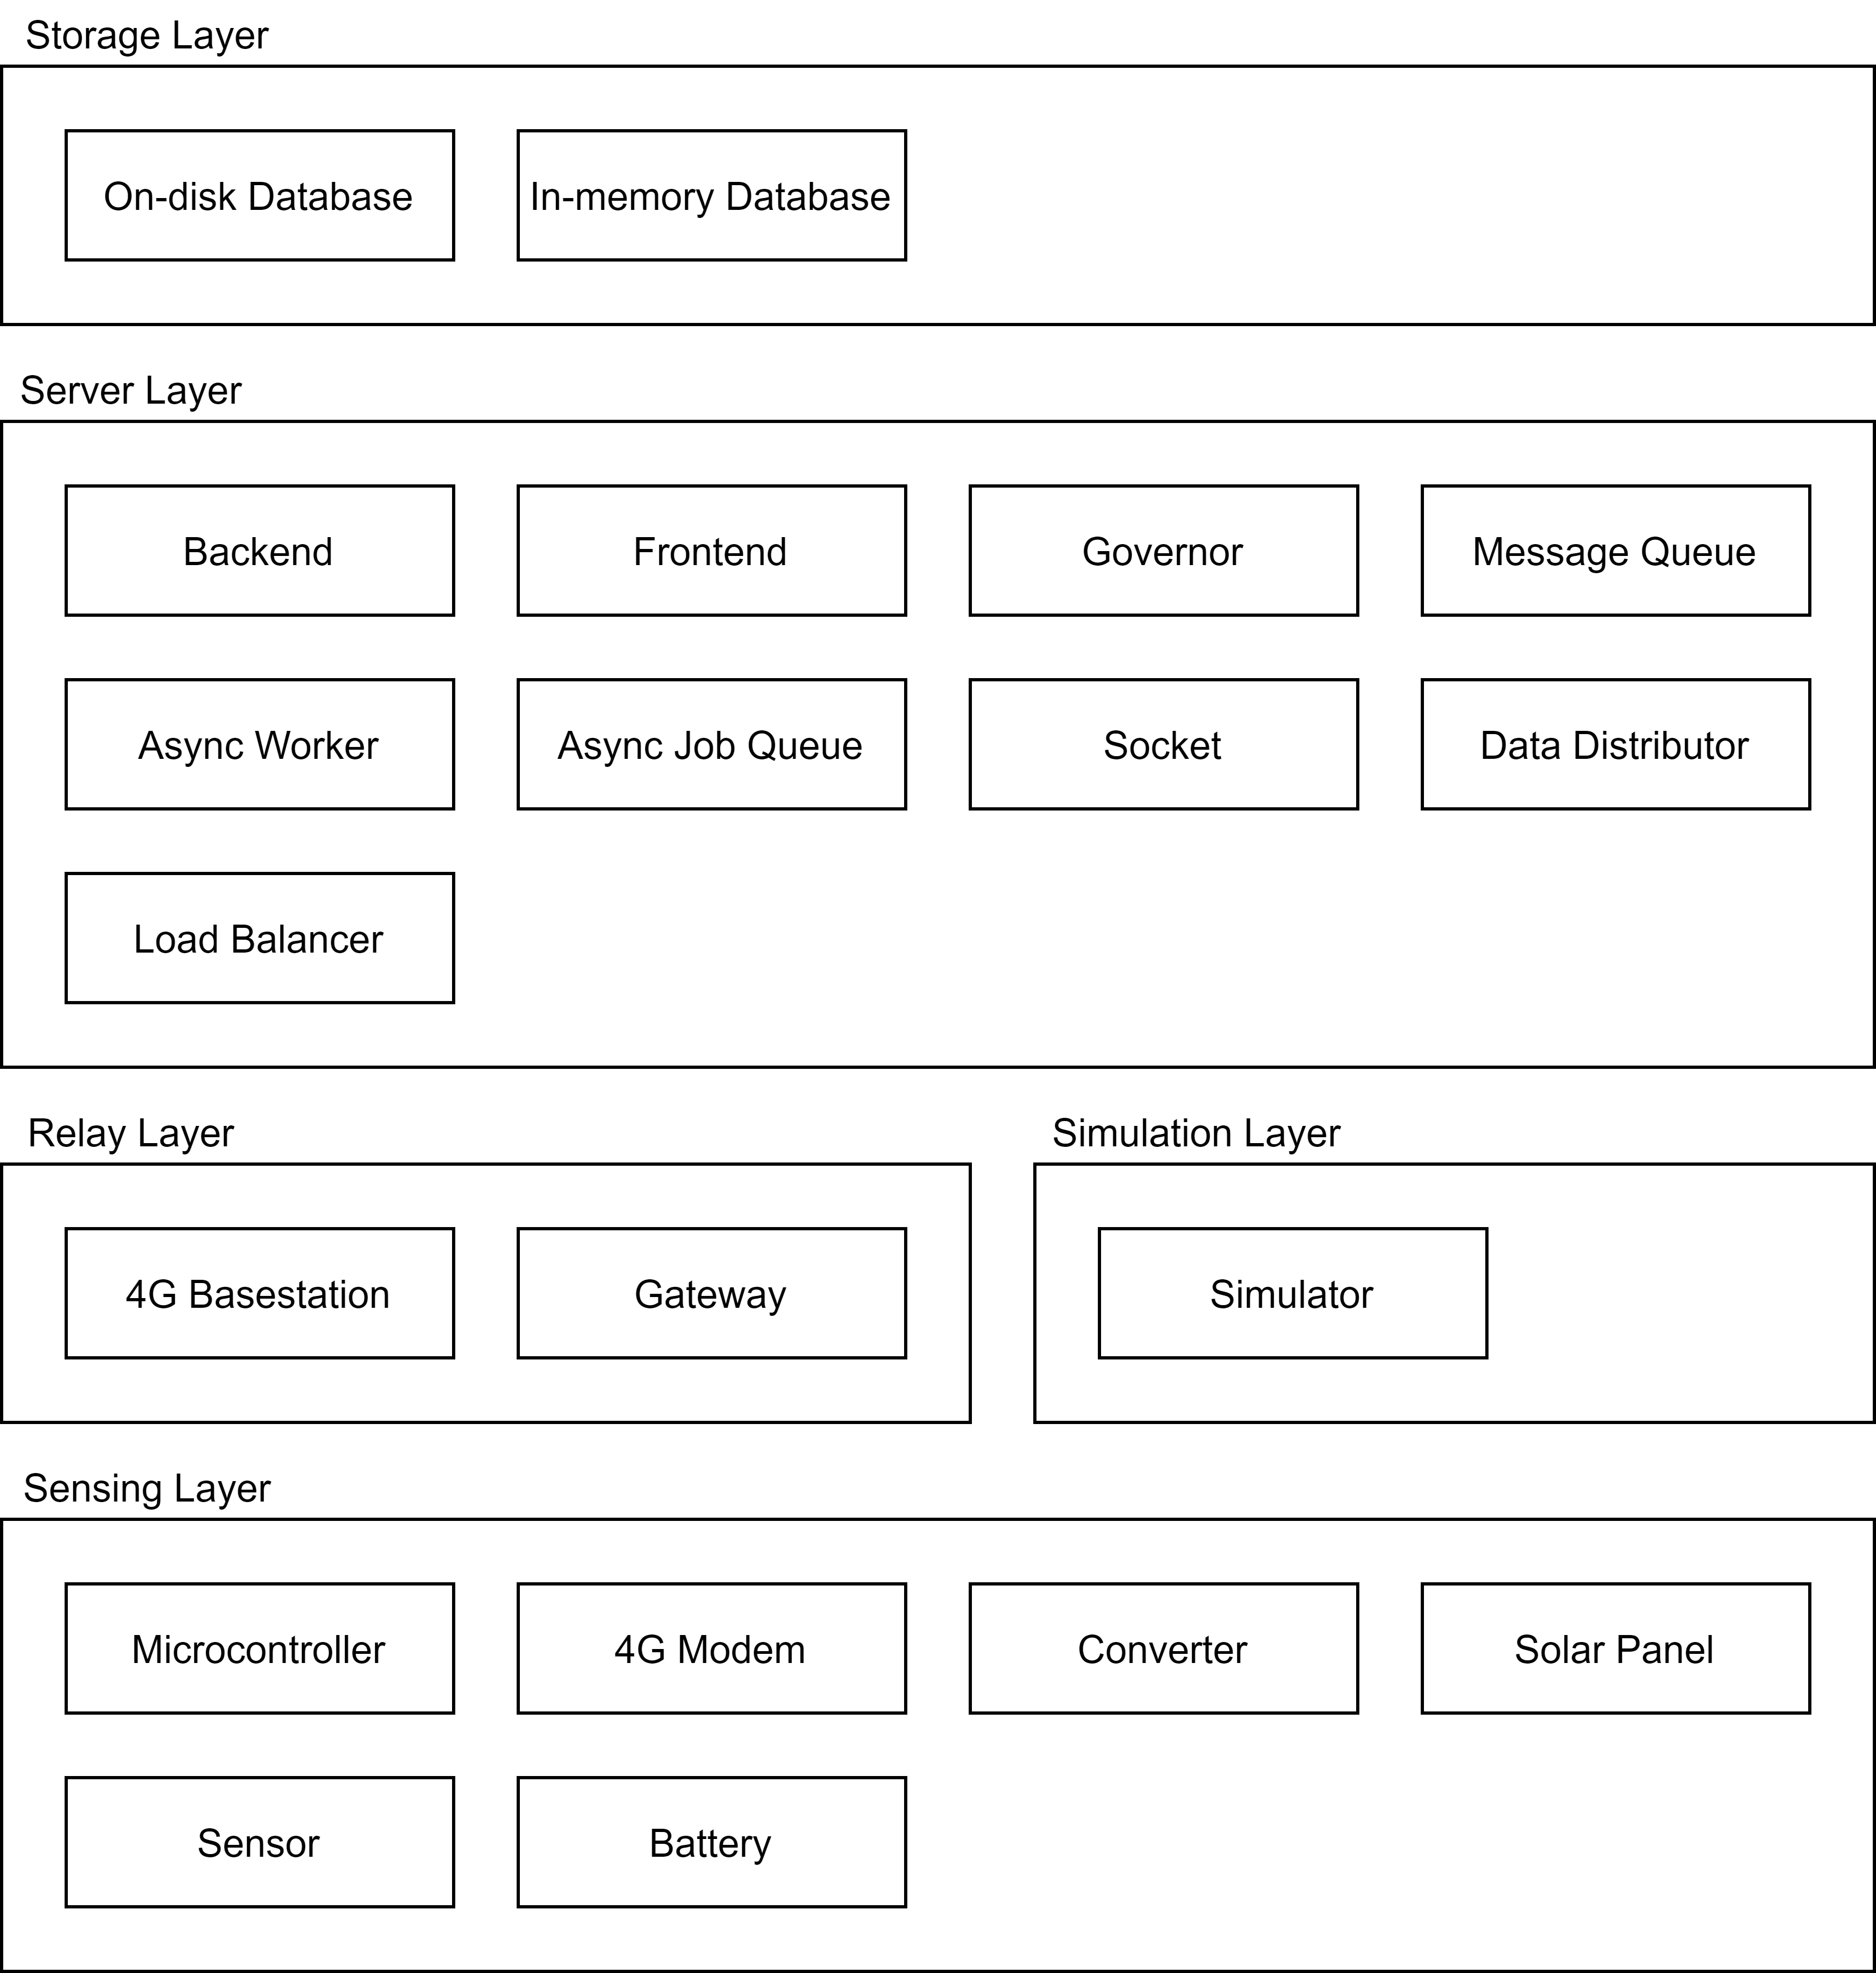
\includegraphics[width=\linewidth]{c3-concept-1.png}
\caption{Concept of the proposed system for monitoring.}
\label{fig:concept1}
\end{figure}


\newpage
\subsection{Controlling}
The lifecycle of command begins at the client-initiated by the user. The command can be anything from setting the output voltage, to shutting down the converter. Once initiated, the client contacts the server to let it know a command had been issued, and the server store it in the database.

On the other hand, the microcontroller performs periodic polling, that is, querying the server if there are new commands issued by the user every second. Similar to the monitoring, the query that is sent from the microcontroller to the server and the reply of the server that is consisting of a list of new commands are transmitted over the 4G cellular network. Finally, the commands are received by the microcontroller and the changes are applied to the converter. The concept of control is shown in figure \ref{fig:concept3}.

\begin{figure}[!ht]
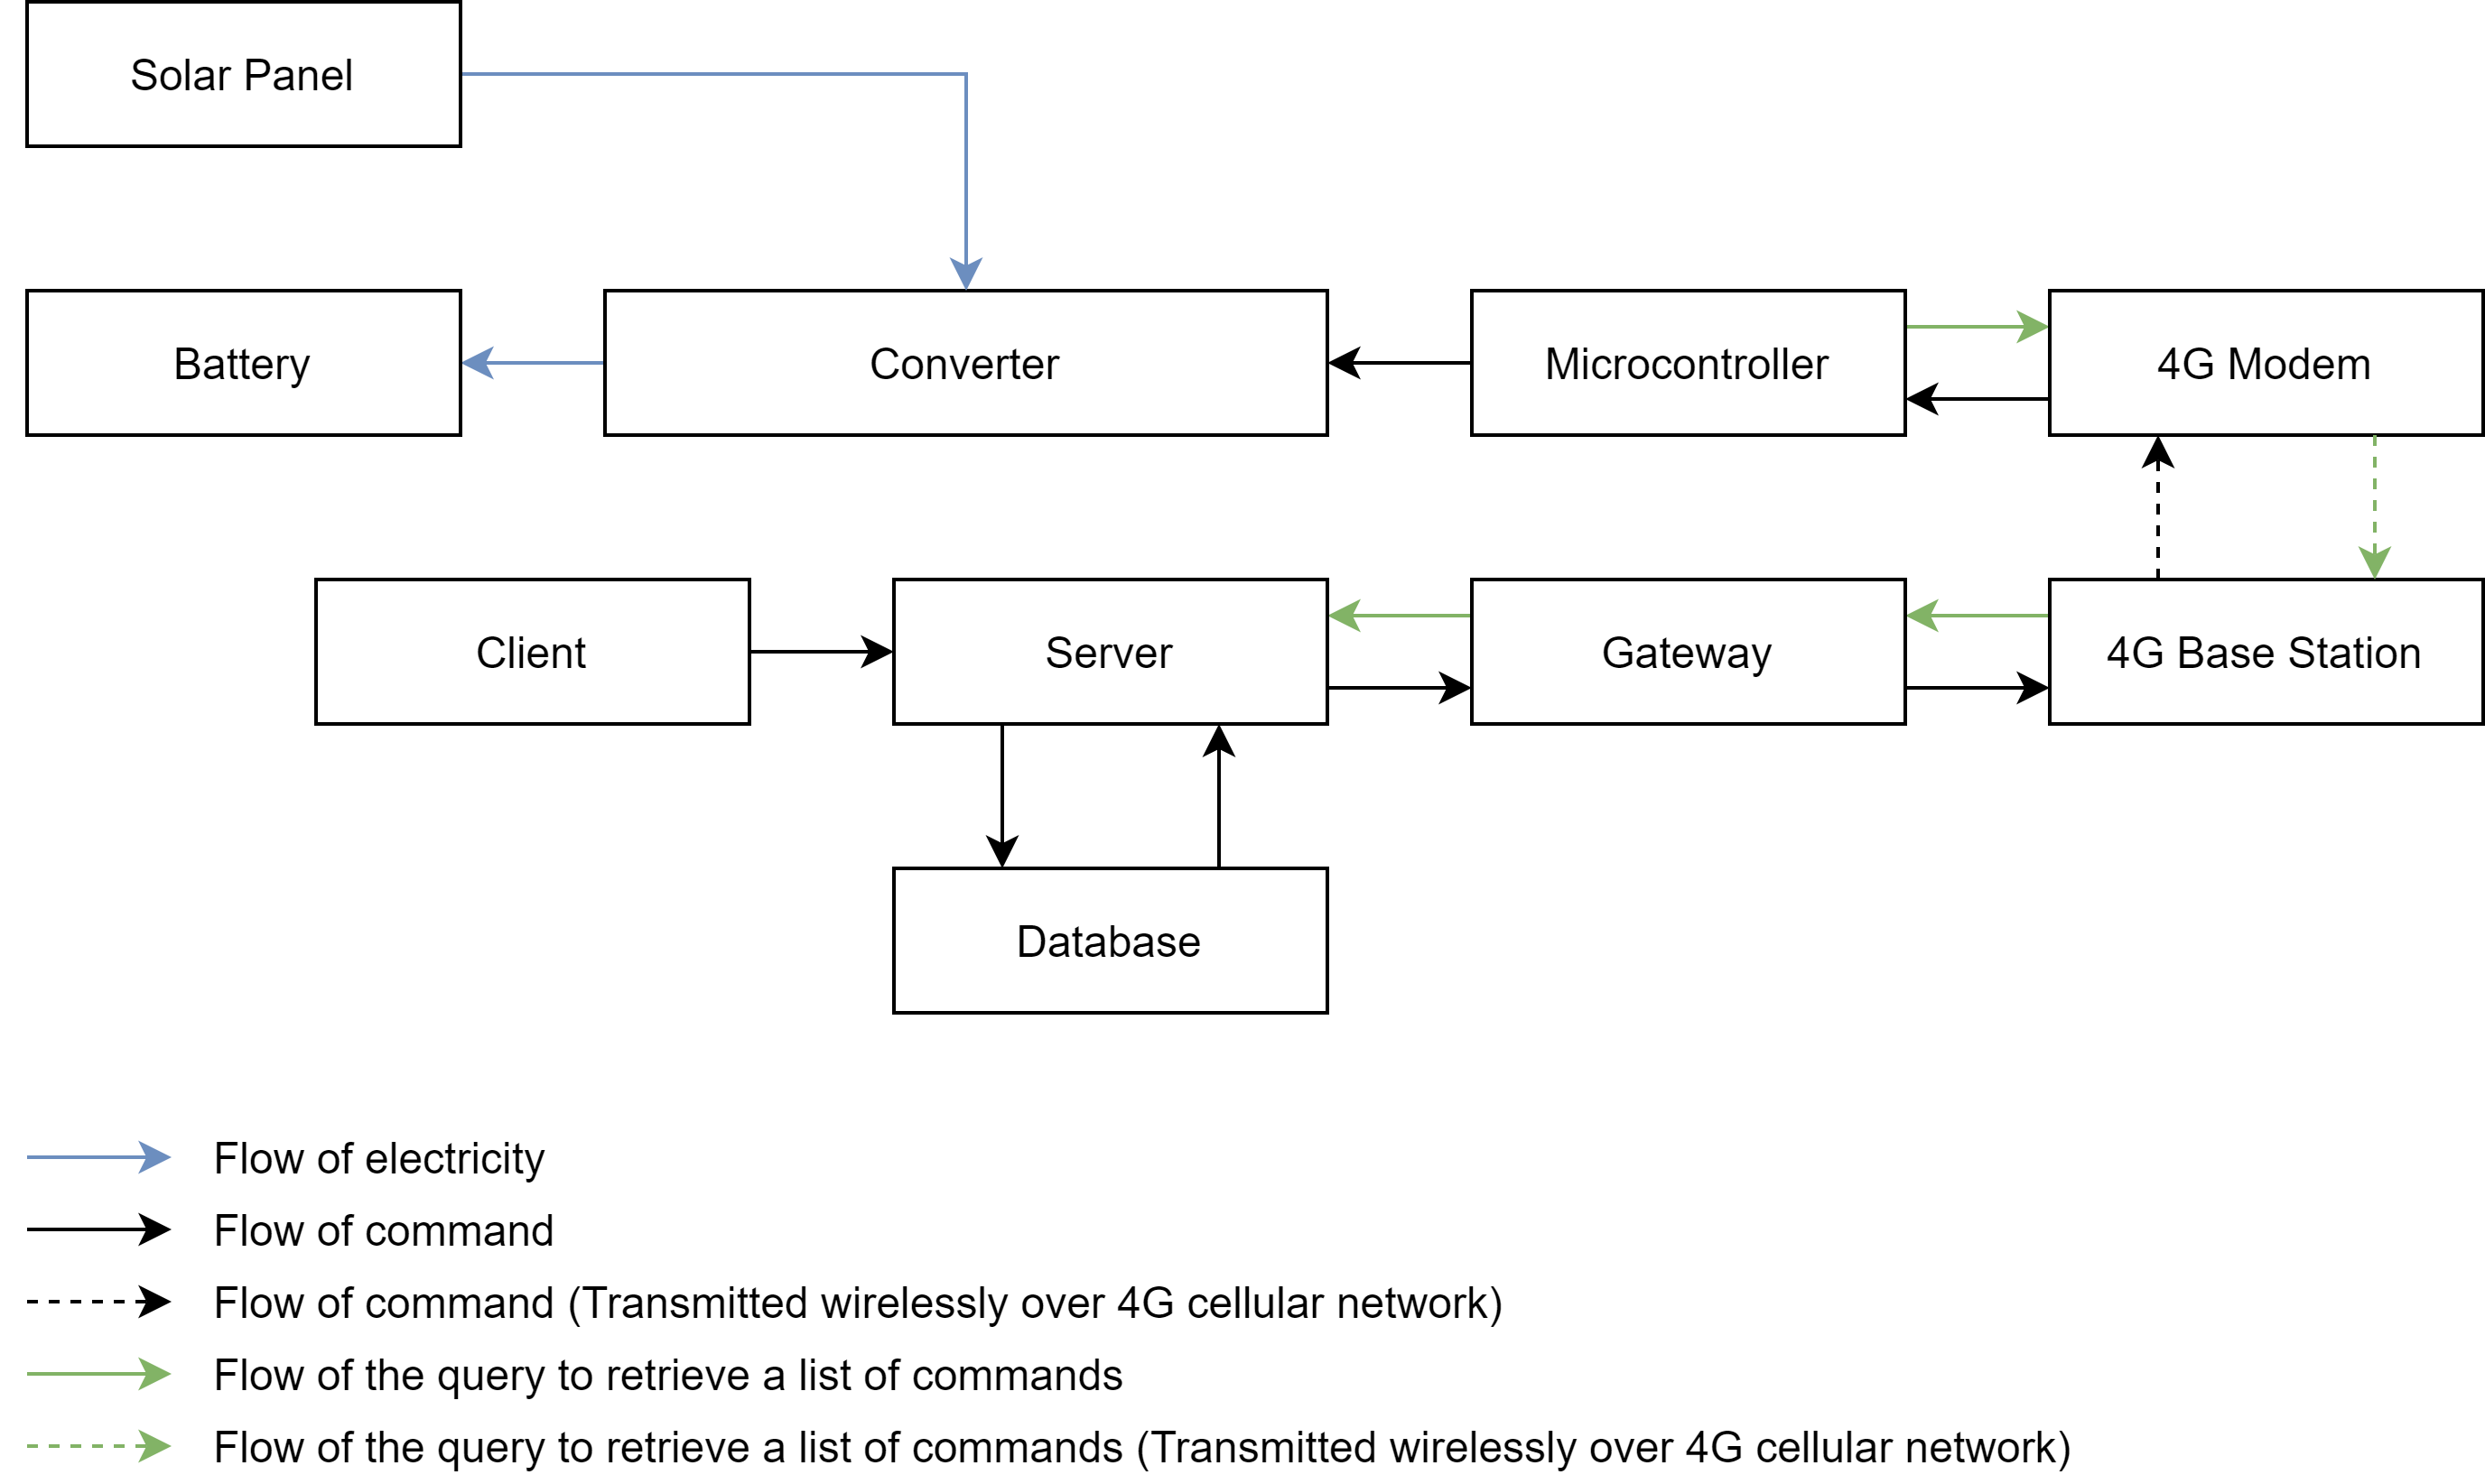
\includegraphics[width=\linewidth]{c3-concept-3.png}
\caption{Concept of the proposed system for controlling.}
\label{fig:concept3}
\end{figure}


\newpage
\section{Layers and components}
\label{sec:layers}

The proposed system is composed of five layers separated by responsibilities. They are:

\begin{itemize}
\item Storage Layer
\item Server Layer
\item Relay Layer
\item Simulation Layer
\item Sensing Layer
\end{itemize}

The storage layer is responsible for storing the state of the server and sensing data received from the microcontrollers. The server layer is where the data processing logic, system monitoring, and data visualisation services are located. The relay layer contains the 4G infrastructures and providing internet access to 4G enabled devices. The sensing layer is responsible for measuring the data and control the generation of power. Lastly, the simulation layer is used to simulate the behaviours of the sensing layer for benchmarking purposes. Figure \ref{fig:concept2} shows the layers and the components within each layer.


\begin{figure}[!ht]
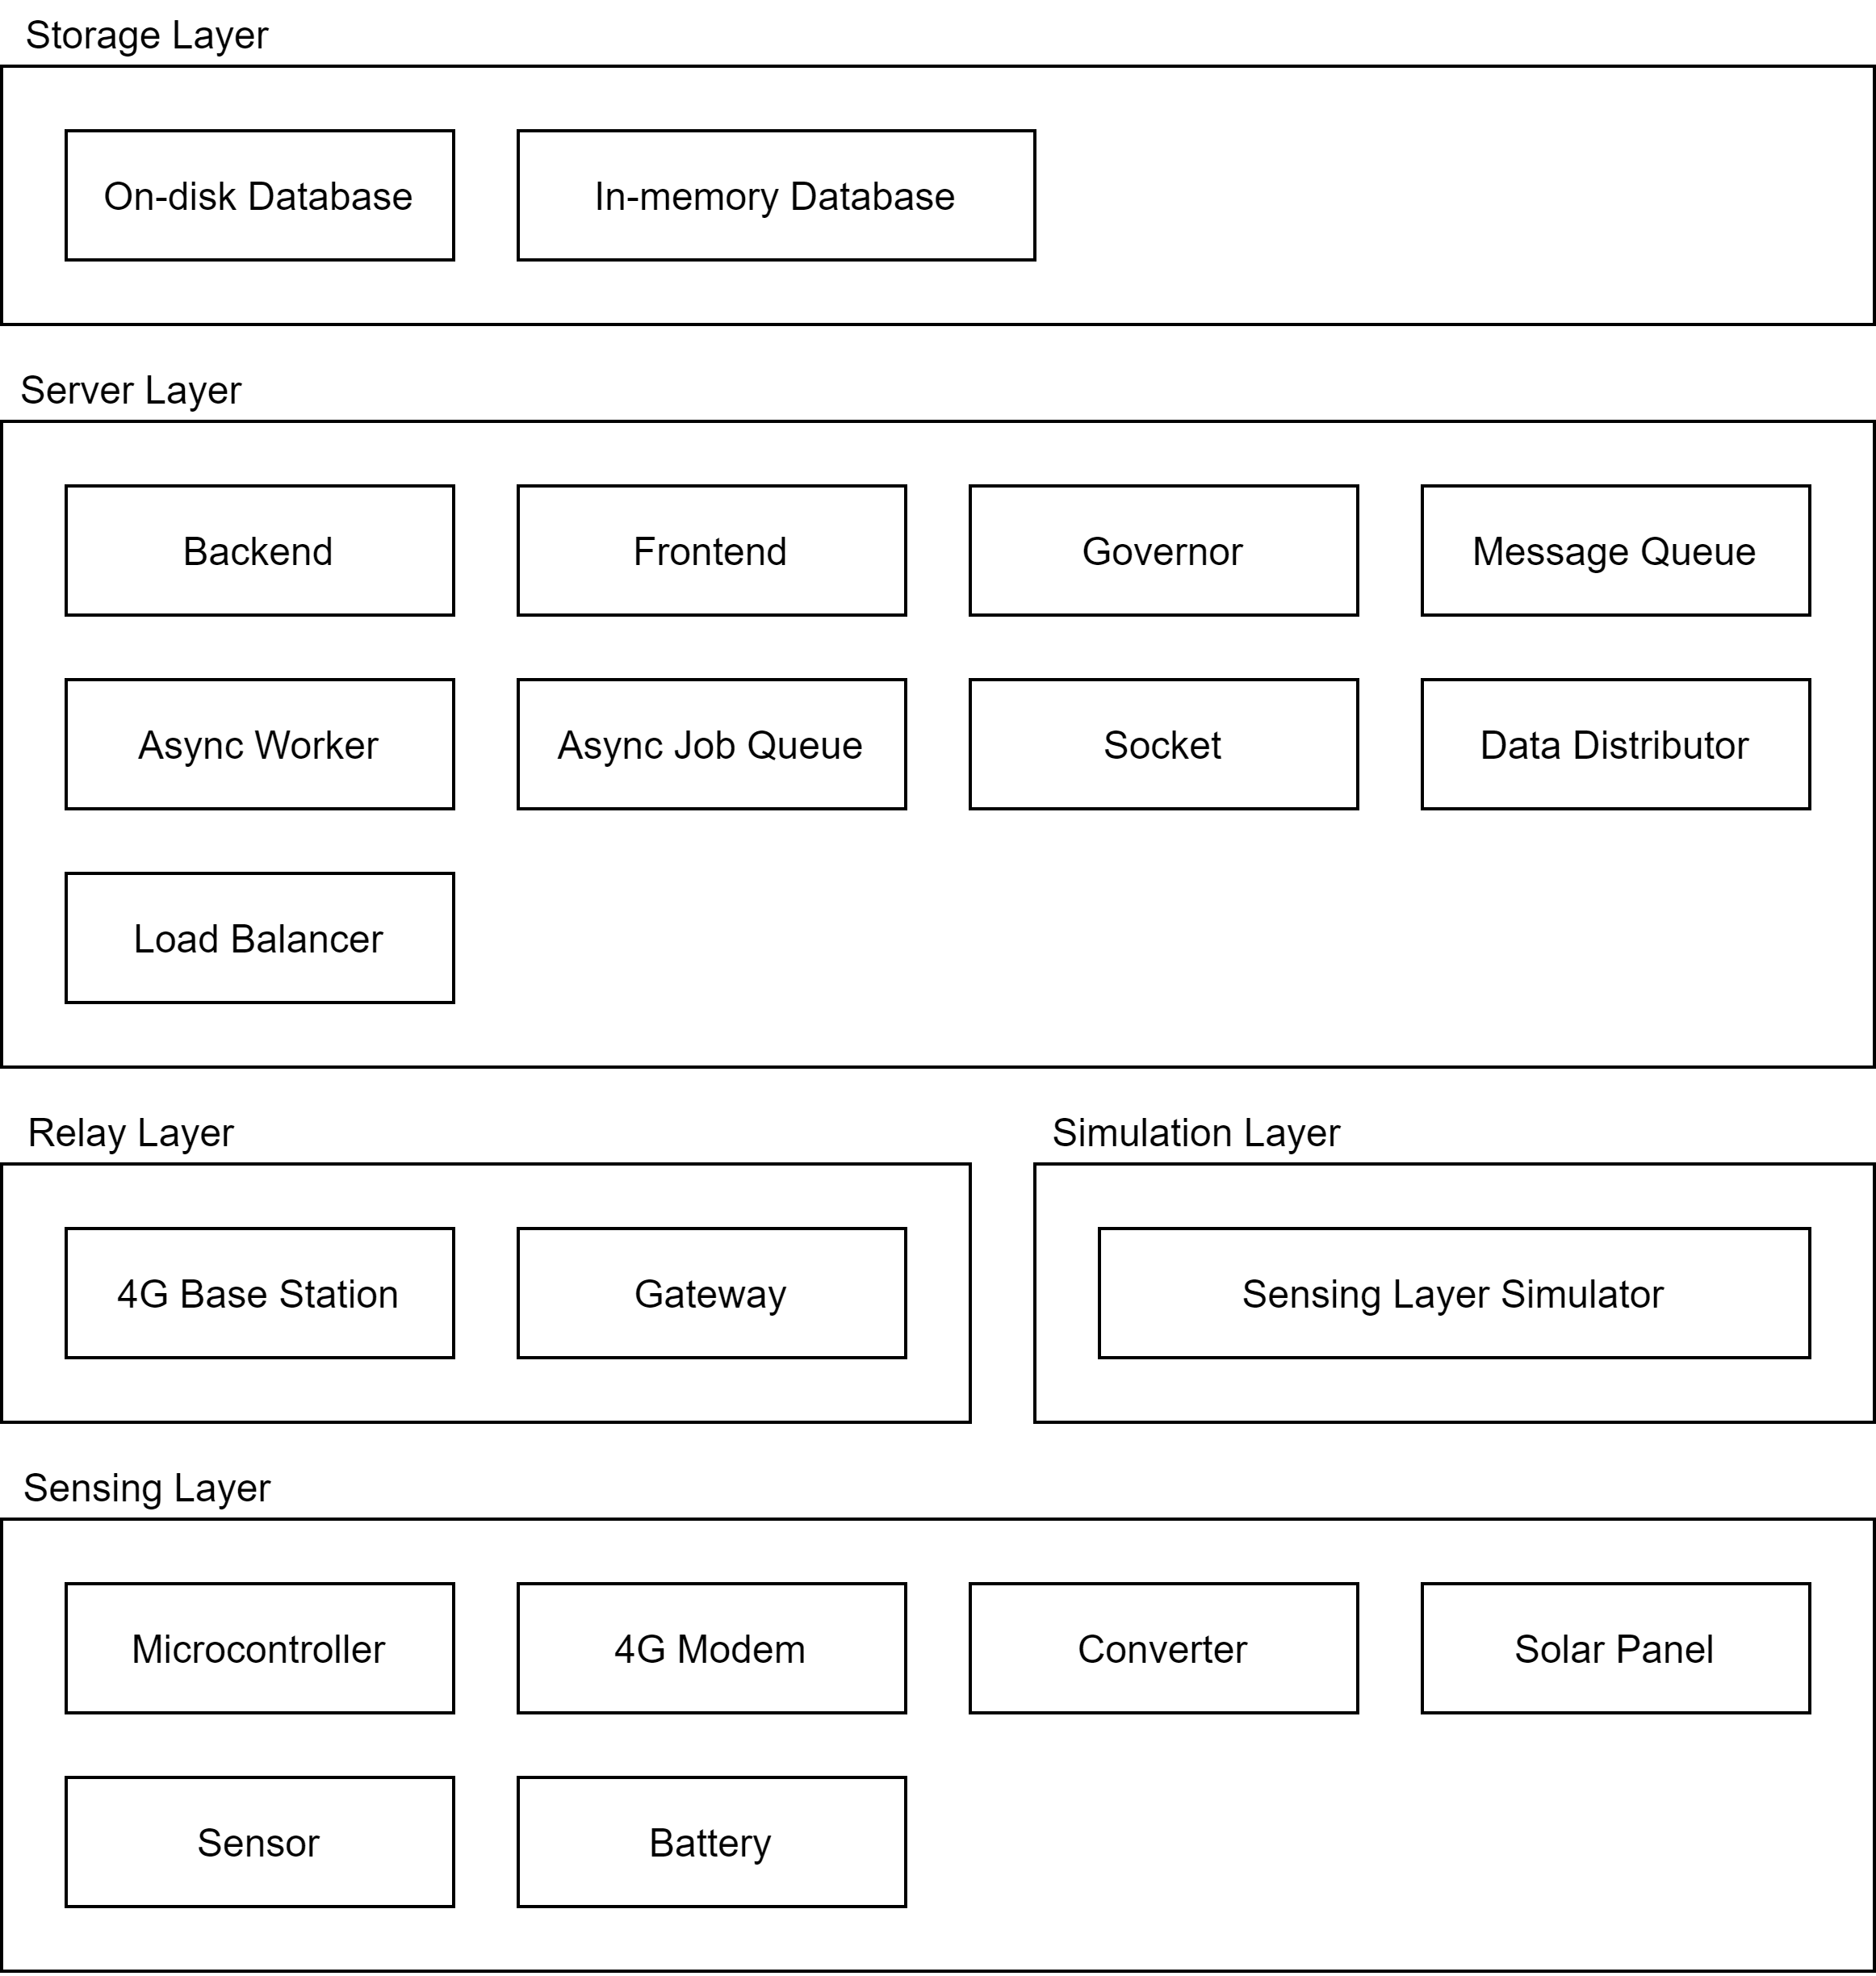
\includegraphics[width=\linewidth]{c3-concept-2.png}
\caption{Layers and components of the proposed system.}
\label{fig:concept2}
\end{figure}

\section{Responsibilities}
\label{sec:responsibilities}

In this section, the responsibilities of each component are described.

\subsection{Storage layer}

\subsubsection{On-disk database}

The distinguishing characteristic of this type of database is the data that is stored in the database is persistent, which means the data remain intact even if the database is down due to failures. It is usually used to store a large amount of data reliably. The downside of using an on-disk database is the response time of querying and inserting data into the database can be very slow. The primary usage in the proposed system is storing the information, status, and sensing data of a device such as a solar panel persistently.

\subsubsection{In-memory database}

The goal for this type of database is not storing the data persistently but aiming to access, modify, and insert data as quick as possible. This advantage is the result of using the memory instead of the disk of the server, which is significantly faster. However, it also comes with the problem of having a significantly smaller capacity, and the data is volatile. That is, the data is gone when the database is down and the data may be purged if the memory of the server is running low. This is primarily used to synchronise the state and sharing data between backend instances that are running on the same server.

\subsection{Server layer}

\subsubsection{Backend}

Backend is a stateless HTTP server and its responsibilities are:

\begin{itemize}
\item Providing application programming interface (API) for microcontrollers to register itself, insert sensing data to the database, and retrieve issued commands.
\item Providing API for the frontend to retrieve data for visualisation and notifying a command had been issued.
\item Providing context-aware load balancing for frontend's real-time data visualisation.
\end{itemize}

\subsubsection{Frontend}

The frontend is a web application and its responsibilities are:

\begin{itemize}
\item Providing a pleasant and usable user interface.
\item Providing real-time data visualisation.
\item Providing a control panel for issuing commands.
\end{itemize}

\subsubsection{Load balancer}

It is a piece of software that distribute the incoming requests to the server instance with the least amount of load. It also uses multiple threads to serve the frontend web pages to improve the performance under load.

\subsubsection{Governor}

The governors are daemons for housekeeping. That is, they are processes that are running in the background of the server and performing some predefined tasks periodically. There is only one governor in the proposed system, its called the data aggregation governor and its job is aggregating the real-time data every minute.

\subsubsection{Message queue}

This is an asynchronous communication system between the components of the server layer. The main contribution of the message queue is enabling processes such as backend, governor, and data distributor to communicate with each other despite they are completely separate programs.

The message queue is asynchronous because the originating process can send a message and continue to perform other tasks without waiting for the message to arrive or a reply is received. As oppose to synchronous communication, where the originating process would stop doing any work and waiting for a reply to receive before continuing.

\subsubsection{Async job queue and worker}

The asynchronous job queue is a queue of tasks to be executed in a first in first out fashion, and the worker is a thread that takes a job from the queue in order and executes them. The backend is using this mechanism to process lengthy but not time-sensitive tasks such as inserting data into the database to improve performance. Similar to the message queue, the originating process adds a job to the queue and it continues to perform other work without waiting for the work to finish.

\subsubsection{Socket}

The socket is the key to efficient real-time communication between the backend and the frontend. This is the enabling technology which allows the frontend to wait for new data to be available as opposed to letting the clients asking for new data every second, which is very inefficient.

\subsubsection{Data distributor}

The data distributor sits between the clients and the backend during the real-time communication. Its purpose is reducing the load of the server by publishing the data to the relevant clients directly.

Without the data distributor, the clients would be notified when a new data is available, and all clients would query the backend for the same piece of data, causing the backend to be accessed directly proportional to the number of clients. By using the data distributor, the data is distributed directly to the clients and no backend access is needed. Note that the data distributor also knows what data each client want and only distribute the data to the clients interested in the data.

\subsection{Relay layer}

This layer contains two key infrastructures, the 4G base station, and the internet gateway. The 4G base station allows 4G enabled devices to communicate with it and forward the data to its internet gateway so that devices can access the internet wirelessly.

\subsection{Sensing layer}

This layer contains power generation devices such as solar panels, power converters, and batteries in our experimental setup. There are also monitoring devices such as sensors that are attached to the input and output of the converter and send analogue signals to the microcontroller. Then, the microcontroller process those signals and send the data to the server over the 4G cellular network using the 4G modem.

\subsection{Simulation layer}

This layer is used for benchmarking as it can generate any number of virtual solar panels and push simulated data to the server. This enables the performance and characteristics of the system to be measured and this layer should behave identically to the sensing layer from the server layer's point of view.

\newpage
\section{Hardware}

The table \ref{tab:hardwareList} outlines the hardware that had been used in the system. Details of each hardware can be found in the subsections below.

\begin{table}[h!]
\begin{center}
\caption{List of hardware in the proposed system.}
\label{tab:hardwareList}
\begin{tabular}{l|l}
\toprule
\textbf{Type} & \textbf{Hardware Model}\\
\midrule
Benchmarking server & Custom Built Desktop (See \autoref{sec:benchmarkingServer})\\
Deployment server & AWS EC2 T2-Medium\\
Microcontroller & Nuvoton M263A\\
4G Modem & Quectel EC25\\
4G Antenna & Antenova SRFL029\\
4G Base Station & Depending on the service provider\\
Gateway & Depending on the service provider\\
Converter & Morningstar PS-MPPT-40M\\
Sensor & ACS723 and ACS724\\
Battery & Sun Xtender PVX-890T\\
\bottomrule
\end{tabular}
\end{center}
\end{table}

\subsection{Benchmarking server}
\label{sec:benchmarkingServer}

This is the server that is being used to benchmark the proposed communication system. The technical specification is detailed in the table \ref{tab:benchmarkingHardware}.

\begin{table}[h!]
\begin{center}
\caption{Technical specification of the benchmarking server.}
\label{tab:benchmarkingHardware}
\begin{tabular}{l|l}
\toprule
\textbf{Name} & \textbf{Specification}\\
\midrule
CPU & AMD Ryzen 3800X (8 Core 16 Threads at 4.3 Ghz)\\
GPU & Nvidia GTX 1080Ti\\
Memory & 16GB 3200Mhz\\
Disk & 4TB HDD + 512GB SSD\\
\bottomrule
\end{tabular}
\end{center}
\end{table}

\subsection{Deployment server}
\label{sec:deploymentServer}

This is the server that is hosted on the AWS cloud computing platform and it is used to deploy the proposed system so that it can be accessed publically. The technical specification is detailed in the table \ref{tab:deploymentHardware}. Note that it is not necessary to deploy the proposed system to a powerful cloud server as there is only one solar panel used for real-world testing.

\begin{table}[h!]
\begin{center}
\caption{Technical specification of the deployment server.}
\label{tab:deploymentHardware}
\begin{tabular}{l|l}
\toprule
\textbf{Name} & \textbf{Specification}\\
\midrule
Instance Type & T2.Medium\\
CPU & 2 Cores\\
Memory & 4GB\\
Disk & 32GB\\
\bottomrule
\end{tabular}
\end{center}
\end{table}


\subsection{Microcontroller}

The selected microcontroller is Nuvoton's M263A. The critical features for this microcontroller that are relevant to the proposed system are shown in the table \ref{tab:microcontrollerSpecification}. See figure \ref{fig:m263A} and \ref{fig:m263Aback} for additional details of the microcontroller.

\begin{table}[h!]
\begin{center}
\caption{Critical features of Nuvoton M263A}
\label{tab:microcontrollerSpecification}
\begin{tabular}{l|l}
\toprule
\textbf{Criteria} & \textbf{Specification}\\
\midrule
CPU & ARM Cortex M23 64MHz\\
APROM Memory & 512KB\\
SRAM Memory & 96KB\\
LDROM Memory & 4KB\\
Has PWM Pins & True\\
Has Analog Pins & True\\
Has SIM card slot & True\\
Has 4G modem support & True\\
\bottomrule
\end{tabular}
\end{center}
\end{table}

\subsection{4G modem}

The selected LTE module is Quectel EC25. The technical specification is shown in the table \ref{tab:quectelEC25} and the figure \ref{fig:quectelEC25} shows the LTE module.

\begin{table}[h!]
\begin{center}
\caption{Technical specification of Quectel EC25}
\label{tab:quectelEC25}
\begin{tabular}{l|l}
\toprule
\textbf{Feature} & \textbf{Specification}\\
\midrule
Form factor & mini PCIe\\
Downlink & 150Mbps\\
Uplink & 50Mbps\\
Has LTE & Enabled\\
\bottomrule
\end{tabular}
\end{center}
\end{table}


\subsection{Converter}

The converter used in real-world testing is the Morningstar PS-MPPT-40M. The technical specification is outlined in the table \ref{tab:psmppt40m}. Note that the proposed system is designed to be generic such that any converter would work similarly with the system.

\begin{table}[h!]
\begin{center}
\caption{Technical specification of Morningstar PS-MPPT-40M}
\label{tab:psmppt40m}
\begin{tabular}{l|l}
\toprule
\textbf{Feature} & \textbf{Specification}\\
\midrule
Max Battery Current & 40 Amps\\
Load Current Rating & 30 Amps\\
Nominal Battery Voltage & 12V or 24V\\
Peak Efficiency & 98\%\\
Battery Voltage Range & 10-35 V\\
\bottomrule
\end{tabular}
\end{center}
\end{table}


\subsection{Voltage and current sensor}

Two sensors are being used to read the voltage and current. The ACS723 shown in the table \ref{tab:acs723} is used to measure the input voltage and current, while ACS724 shown in the table \ref{tab:acs724} is used to measure the output voltage and current. Note the input voltage and current are referring to the voltage and current of the electricity flowing from the solar panel to the converter, and the output current and voltage are referring to the voltage and current of the electricity flowing from the converter to the battery. Additionally, the proposed system should work with any sensor with analogue output as long as the parameters in the microcontroller are properly set.

\begin{table}[h!]
\begin{center}
\caption{Technical specification of ACS723 sensor}
\label{tab:acs723}
\begin{tabular}{l|l}
\toprule
\textbf{Characteristic} & \textbf{Specification}\\
\midrule
Sensitivity & Typ. 400 (mV/A)\\
Zero-Current Output Voltage & Typ. VCC * 0.1 (V)\\
\bottomrule
\end{tabular}
\end{center}
\end{table}

\begin{table}[h!]
\begin{center}
\caption{Technical specification of ACS724 sensor}
\label{tab:acs724}
\begin{tabular}{l|l}
\toprule
\textbf{Characteristic} & \textbf{Specification}\\
\midrule
Sensitivity & Typ. 100 (mV/A)\\
Zero-Current Output Voltage & Typ. VCC * 0.5 (V)\\
\bottomrule
\end{tabular}
\end{center}
\end{table}

\newpage
\subsection{Battery}

The battery model used in real-world testing is Sun Xtender PVX-890T. The technical specification for the battery is shown in the table \ref{tab:pvx890t}.

\begin{table}[h!]
\begin{center}
\caption{Technical specification of Sun Xtender PVX-890T}
\label{tab:pvx890t}
\begin{tabular}{l|l}
\toprule
\textbf{Characteristic} & \textbf{Specification}\\
\midrule
Nominal Voltage & 12 Volt\\
Ampere Hour Capacity @ 24 Hour Rate & 89\\
Bulk/Absorb Charge & 14.2-14.4 Volts\\
Float Charge & 13.2-13.4 Volts\\
\bottomrule
\end{tabular}
\end{center}
\end{table}

\subsection{Solar Panel}

The solar panel used in real-world testing is Suntellite ZDNY-260p60. The technical specification for the solar panel in shown in the table \ref{tab:solarpanel}.

\begin{table}[h!]
\begin{center}
\caption{Technical specification of Suntellite ZDNY-260p60}
\label{tab:solarpanel}
\begin{tabular}{l|l}
\toprule
\textbf{Characteristic} & \textbf{Specification}\\
\midrule
Power & 260W\\
$V_{mpp}$ & 30.73V\\
$I_{mpp}$ & 8.47A\\
$V_{oc}$ & 37.9V\\
$I_{sc}$& 9.01A\\
Efficiency& 15.98\%\\
\bottomrule
\end{tabular}
\end{center}
\end{table}


\section{Software}
\label{sec:software}

The table \ref{tab:softwareList} outlines the software that had been used in the system and their responsibilities are outlined in the \autoref{sec:responsibilities}.

\begin{table}[h!]
\begin{center}
\caption{List of software in the proposed system.}
\label{tab:softwareList}
\begin{tabular}{l|l}
\toprule
\textbf{Component} & \textbf{Software}\\
\midrule
Benchmarking operating system & Ubuntu Desktop 20.04 LTS\\
Deployment operating system & Ubuntu Server 20.04 LTS\\
Microcontroller platform & Mbed OS 15.5\\
Message queue & Apache Pulsar\\
Job queue and worker & RedisRQ\\
Frontend & ReactJS and nivo.rock\\
Backend & Python Flask\\
Socket & socket.io\\
Load Balancer & nginx\\
WSGI Server & Gunicorn\\
On-disk Database & MongoDB\\
In-memory Database & Redis\\
Programming language & Python 3.6\\
\bottomrule
\end{tabular}
\end{center}
\end{table}

\section{Cost estimate}

The cost of the microcontroller that is being used in the thesis is shown in the table \ref{tab:mcestimateexp}. Note that there are many other modules such as Wi-Fi, LoRaWAN, Bluetooth, accelerometer, temperature sensor, etc. included in the price of the microcontroller which is not necessary for the proposed system to work. Additionally, the cost listed in the table is based on the retail price, not the wholesale price.

\begin{table}[h!]
\begin{center}
\caption{The cost of the microcontroller in the experimental setup.}
\label{tab:mcestimateexp}
\begin{tabular}{l|l}
\toprule
\textbf{Component} & \textbf{Retail price}\\
\midrule
EC25 LTE Modem (mini PCIe) & 69 AUD\\
Nuvoton M263A & 143 AUD\\
Antenova SRFL029 & 10 AUD\\
ACS723 Sensor & 16 AUD\\
ACS724 Sensor & 14 AUD\\
\midrule
Total & 252 AUD or 177 USD\\
\bottomrule
\end{tabular}
\end{center}
\end{table}

The table \ref{tab:mcestimate} shows a rough cost estimate for a microcontroller that supports LTE cellular network, PWM output, analogue input, and preferably 50Mhz or higher processor clock speed. The cost estimate only shows the cost of the critical components of the microcontroller and miscellaneous cost is not included as they are design dependent.

\begin{table}[h!]
\begin{center}
\caption{Cost estimate of a microcontroller that meets the minimum requriements.}
\label{tab:mcestimate}
\begin{tabular}{l|l}
\toprule
\textbf{Component} & \textbf{Retail price}\\
\midrule
Sierra HL Series LTE Modem (LLC) & 22 AUD\\
M2351KIAAE Processor & 5 AUD\\
Antenova SRFL029 & 10 AUD\\
ACS723 Sensor (LLC) & 6.5 AUD\\
ACS724 Sensor (LLC) & 4.5 AUD\\
\midrule
Total & 48 AUD or 33 USD\\
\bottomrule
\end{tabular}
\end{center}
\end{table}

\end{document}